\documentclass[9pt]{beamer}
\usetheme{boxes}
\usetheme{Boadilla}
\usecolortheme{beaver}
%\usecolortheme{sidebartab}
% \usefonttheme{structurebold}
\usefonttheme{serif}


% \usepackage{helvet}
\usepackage{amsmath, amssymb}
\usepackage{color}
%\usepackage{asymptote}
\usepackage{mathrsfs}
\usepackage{dsfont}
\usepackage{url}
\usepackage{cancel}
\usepackage{tikz}
\usetikzlibrary{fit,positioning}
\usetikzlibrary{shapes,matrix,decorations.markings,arrows}
\usetikzlibrary{graphs}


%
%
%\newcommand{\LABEQ}[1]{\label{eq:#1}}%\mathtt{[eq:#1]}\qquad
%\newcommand{\LABALG}[1]{\label{alg:#1}}%\mathtt{[lab:#1]}\qquad
%\newcommand{\LABTAB}[1]{\label{tab:#1}}%{\tt [tab:$\text{$#1$}$]}}
%\newcommand{\LABFIG}[1]{\label{fig:#1}}%{\tt [fig:$\text{$#1$}$]}}
%\newcommand{\LABTHM}[1]{\label{thm:#1}}%{\tt [thm:#1]}}
%\newcommand{\LABPRP}[1]{\label{prp:#1}}%{\tt [prp:#1]}}
%\newcommand{\LABLEM}[1]{\label{lem:#1}}%{\tt [lem:#1]}}
%\newcommand{\LABCOR}[1]{\label{cor:#1}}%{\tt [cor:#1]}}
%\newcommand{\LABDFN}[1]{\label{dfn:#1}}%{\tt [dfn:#1]}}
%\newcommand{\LABFNT}[1]{\label{fnt:#1}}%{\tt [fnt:#1]}}
%\newcommand{\EQ}[1]{\eqref{eq:#1}}%$^{\text{\tt [#1]}}$} %used to be  %{(\ref{eq:#1})}
%\newcommand{\ALG}[1]{~\ref{alg:#1}}
%\newcommand{\TAB}[1]{~\ref{tab:#1}}%$^{\text{\tt [#1]}}$}
%\newcommand{\FIG}[1]{\ref{fig:#1}} %$^{\text{\tt [#1]}}$}
%\newcommand{\THM}[1]{~\ref{thm:#1}}%$^{\text{\tt [#1]}}$}
%\newcommand{\COR}[1]{~\ref{cor:#1}}%$^{\text{\tt [#1]}}$}
%\newcommand{\PRP}[1]{~\ref{prp:#1}}%$^{\text{\tt [#1]}}$}
%\newcommand{\LEM}[1]{~\ref{lem:#1}}%$^{\text{\tt [#1]}}$}
%\newcommand{\DFN}[1]{~\ref{dfn:#1}}%$^{\text{\tt [#1]}}$}
%\newcommand{\FNT}[1]{~\ref{fnt:#1}}%$^{\text{\tt [#1]}}$}
%\newcommand{\PAGEEQ}[1]{~\pageref{eq:#1}}
%\newcommand{\PAGETAB}[1]{~\pageref{tab:#1}}
%\newcommand{\PAGEFIG}[1]{~\pageref{fig:#1}}
%\newcommand{\LABCHAP}[1]{\label{chap:#1}}%{\tt [chap:#1]}}
%\newcommand{\LABSEC}[1]{\label{sec:#1}}%{\tt [sec:#1]}}
%\newcommand{\LABSSEC}[1]{\label{ssec:#1}}%{\tt [ssec:#1]}}
%\newcommand{\LABSSSEC}[1]{\label{sssec:#1}}%{\tt [sssec:#1]}}
%\newcommand{\CHAP}[1]{~\ref{chap:#1}}%$^{\text{\tt [c:#1]}}$}
%\newcommand{\SEC}[1]{~\ref{sec:#1}}%$^{\text{\tt [s:#1]}}$}
%\newcommand{\SSEC}[1]{~\ref{ssec:#1}}%$^{\text{\tt [ss:#1]}}$}
%\newcommand{\SSSEC}[1]{~\ref{sssec:#1}}%$^{\text{\tt [sss:#1]}}$}
%
\definecolor{darkblue}{rgb}{0.0, 0.0, 0.45}
\setbeamercolor{title}{fg=darkblue}
\setbeamercolor{frametitle}{fg=darkblue}
\newcommand{\myitem}{\item[$\bullet$]}

%gets rid of bottom navigation bars
\setbeamertemplate{footline}[page number]{}

%gets rid of navigation symbols
\setbeamertemplate{navigation symbols}{}

\newcommand{\ve}[1]{\boldsymbol{#1}}
\def\X{\ve{X}}
\def\x{\ve{x}}
\def\hx{\hat{\x}}
\def\m{\ve{m}}
\def\y{\ve{y}}
\def\G{\ve{G}}
\def\H{\ve{H}}
\def\C{\mathcal{C}}
\def\O{\mathcal{O}}
\def\b{\ve{b}}
\def\E{\mc{E}}
\def\R{\mc{R}}



\def\pe{{\varepsilon}}
\def\n{{\mathtt{n}}}
\def\nn{{\nonumber}}
\def\rate{{\mathtt{r}}}

%Original left degree distribution
\def\lambimax{{l_{\text{max}}}}				       %maximun lambda degree
\newcommand{{\Tlmax}}[1]{\lambimax(#1)}      %maximun left degree  (t)
\newcommand{\lambi}[1]{\lambda_{#1}}		%lambda_i
\newcommand{\lamb}[1]{\lambda(#1)}		%lambda(x),lambda(t)
\def\lambfull{{\lamb{x}=\sum_{i=1}^{\lambimax}\lambi{i}x^{i-1}}} %Full expression of lambda(x)
\def\lavg{{l_{\text{avg}}}}						%lavg
\newcommand{\lav}[1]{\lavg(#1)}			%lavg(t)

%Original right degree distribution
\def\rhimax{{r_{\text{max}}}}
\newcommand{\rhi}[1]{\rho_{#1}}
\newcommand{\rh}[1]{\rho(#1)}
\def\rhofull{{\rh{x}=\sum_{j=1}^{\rhimax}\rhi{j}x^{j-1}}}
\def\ravg{{r_{\text{avg}}}}
\newcommand{\rav}[1]{\ravg(#1)}



\newcommand{\mc}[1]{\mathcal{#1}}
\def\sX{\mc{X}}
\def\N{\mc{N}}
\newcommand{\mxf}[3]{m^{#3}_{X_{#1}\rightarrow f_{#2}}(x_{#1})}
\newcommand{\mfx}[3]{m^{#3}_{f_{#2}\rightarrow X_{#1}}(x_{#1})}

\newcommand\Def[1]{{\textbf{\textcolor{DeepSkyBlue4}{Definition:}}\\\emph{#1}\\\begin{center} \textcolor{DeepSkyBlue4}{------------------------} \end{center}}}
\newcommand\Prop[1]{{\textbf{\textcolor{red}{Property:}}\\\emph{#1}\\\begin{center} \textcolor{red}{------------------------} \end{center}}}



\newcommand{\fs}[2]{#2}

\title[]{Low-density Parity-Check Codes \\ Over the Binary Erasure Channel}
\author[\textcolor{white}{Advanced Digital Communications}]{Introduction to Graphical Models and Inference for Communications\\\vspace*{3mm}{\small \textcolor{black}{UC3M}}
}
%\date[08/02/2016]{{08/02/2016}}
\institute{\textcolor{white}{}}

% \pgfdeclareimage[height=0.5cm]{ITW}{pics/Logo.png}
%  \logo{\pgfuseimage{ITW}}

\AtBeginSection[]
{
  \begin{frame}<beamer>{Index}
    \tableofcontents[currentsection,currentsubsection]
  \end{frame}
}

\begin{document}

\frame{
\titlepage
\thispagestyle{empty}
\begin{center}
\includegraphics[scale=0.05]{Figuras/uc3m-logo.pdf}
\end{center}
}



%\section{Introduction}

\frame{
\frametitle{Today}

\begin{itemize}
\item Binary Erasure Channel, coding rate and channel capacity.
\item Optimal decoding and the \emph{Classical} coding approach.
\item Modern coding theory in a nutshell. 
\item Introduction to Low-Density Parity Check codes.
\item LDPC Asymptotic analysis for the $(3,6)$-LDPC ensemble.
\end{itemize}



}

\section{BEC}

\frame{
\frametitle{The binary erasure channel (BEC)}

\begin{center}
\includegraphics[scale=0.40]{Figuras/BEC.pdf}
\end{center}

\color{darkblue}{Is not  this channel model too simple??}\color{black}{}

\begin{itemize}
\item Yes! That's why we like it! We can make analytical predictions.
\item \emph{Quite surprisingly, most properties and statements that we encounter in our investigation of LDPC codes over the BEC hold in much greater generality.} (R. Urbanke and T. Richardson, Modern Coding Theory).
\item Erasure correcting codes are used in the link layer of every communication stardard!
\end{itemize}



}

 \frame{
\begin{center}
\includegraphics[scale=0.40]{Figuras/BEC.pdf}
\end{center}



\begin{exampleblock}{Uncoded transmission}
\begin{itemize}
\item Average error probability: $\pe$
\item This is ok if $\pe=10^{-8}\ldots$ what if $\pe=0.5$? 
\end{itemize}
\end{exampleblock}

\begin{block}{Transmission of encoded bits}
\begin{align*}
\underbrace{\m}_{m \text{ information bits }} & \rightarrow \underbrace{\x}_{n \text{ encoded bits }}  \rightarrow \underbrace{\y}_{n \text{ channel observations }} \rightarrow \underbrace{\hat{\x}}_{\text{decoded codeword}}  \\\\
&\rate=\frac{m}{n} \qquad \qquad \text{ (coding rate) }
\end{align*}
\end{block}

}

\frame{

\begin{block}{Transmission of encoded bits}
\begin{align*}
\underbrace{\m}_{m \text{ information bits }} & \rightarrow \underbrace{\x}_{n \text{ encoded bits }}  \rightarrow \underbrace{\y}_{n \text{ channel observations }} \rightarrow \underbrace{\hat{\x}}_{\text{decoded codeword}}  \\
&\rate=\frac{m}{n} \qquad \qquad \text{ coding rate }
\end{align*}
\end{block}

\begin{itemize}
\item If we let $\rate\rightarrow0$, we can easily find a coding scheme such that $P(\hx\neq\x|\y)\rightarrow 0$. E.g. a repetition code
\begin{align*}
m_i\in\{0,1\} \rightarrow \x=\underbrace{[m_i ~ m_i ~ \ldots m_i ]}_{m_i \text{ is repeated $n$ times }}
\end{align*}
\item Problem solved?
\end{itemize}

}

\frame{
\frametitle{BEC  capacity}

\begin{exampleblock}{Channel Capacity}
\begin{align}\nonumber
C=1-\varepsilon
\end{align}
\end{exampleblock}

\begin{itemize}
\item Assume $\pe=0.5$
\item Theoretically, for any $\delta\in(0,0.5)$ there exits a coding scheme  of rate $\rate=0.5-\delta$ for which $P(\hx\neq\x|\y)\rightarrow0$ if we let $\n\rightarrow\infty$
\end{itemize}

\begin{alertblock}{}
We are wasting resources (information transmission rate, energy) if we use $\rate\rightarrow 0$!!
\end{alertblock}

\begin{block}{}
Our goal is to design feasible encoding and decoding schemes that allow us to operate close to channel capacity.
\end{block}

}

\section{Linear Block Codes and MAP decoding}

\frame{
\frametitle{Linear block codes}
\begin{itemize}
\item All codes used in practice (classic and modern) are linear.
\item \textbf{Generator matrix: } $\x=\m\mathbf{G}$ where $\m\in\{0,1\}^{m}$.
\item \textbf{Parity check matrix:} $\x\H^T=\ve{0}~~ \forall \x\in \C$.
\item Each row of the parity check matrix establishes a linear constraint between coded bits.
\end{itemize}

\vspace{0.5cm}
For a Hamming $(7,4)$ code 
\begin{align*}
\G=\left[
\begin{array}{ccccccc}
1 & 1 & 1 & 0 & 0 & 0 & 0 \\
1 & 0 & 0 & 1 & 1 & 0 & 0 \\
0 & 1 & 0 & 1 & 0 & 1 & 0 \\
1 & 1 & 0 & 1 & 0 & 0 & 1 
\end{array}
\right], \quad
\H=\left[
\begin{array}{ccccccc}
1 & 0 & 1 & 0 & 1 & 0 & 1\\
0 & 1 & 1 & 0 & 0 & 1 & 1 \\
0 & 0 & 0 & 1 & 1 & 1 & 1
\end{array}
\right]
\end{align*}
Therefore...
\begin{align*}
&x_1\oplus x_3\oplus x_5\oplus x_7=0\\
&x_2\oplus x_3\oplus x_6\oplus x_7=0\\
&x_4\oplus x_5\oplus x_6\oplus x_7=0
\end{align*}

}

\frame{
\frametitle{Transmission over the BEC}
\begin{itemize}
\item Linear block code $(m,n)$ with $\G$, $\H$ matrices.
\item Codeword $\x$ is sent.
\end{itemize}


\begin{block}{}
\begin{columns}[T]
\begin{column}{0.4\textwidth}
\begin{itemize}
\item Vector $\y$ is observed. 
\item $\mc{E}$ index set of erased bits.
\item $\mc{R}$ index set of received bits.
\item $\E\cup\R=\{1,\ldots,n\}$.
\end{itemize}
\end{column}
\begin{column}{0.6\textwidth}
\begin{center}
\includegraphics[scale=0.40]{Figuras/BEC.pdf}
\end{center}
\end{column}
\end{columns}
\end{block}

Thus, for the BEC
\begin{align*}
\y(\mc{E})=?,\qquad \y(\R)=\x(\R)
\end{align*}

}

\frame{
\frametitle{Optimal decoding over the BEC}

\begin{itemize}
\item Hamming $(7,4)$ code.
\item $\x=\left[
\begin{array}{ccccccc}
1 & 1 & 1 & 0 & 0 & 0 & 0
\end{array}
\right]$
is sent.
\item $\y=\left[
\begin{array}{ccccccc}
1 & ? & 1 & 0 & ? & ? & 0
\end{array}
\right]$ is received.
\item $\E=\{2,5,6\}$ and $\R=\{1,3,4,7\}$.
\end{itemize}

\begin{exampleblock}{}
Thus, the system of equations
\begin{align*}
&x_1\oplus x_3\oplus x_5\oplus x_7=0\\
&x_2\oplus x_3\oplus x_6\oplus x_7=0\\
&x_4\oplus x_5\oplus x_6\oplus x_7=0
\end{align*}
can be simplified to
\begin{align*}
&x_5=0\\
&x_2\oplus x_6=1\\
&x_5\oplus x_6=0
\end{align*}
By solving the system of binary equations we get a unique solution $\hat{\x}=[1 1 1 0 0 0 0 ]=\x$.
\end{exampleblock}
}

\frame{
\begin{itemize}
\item Linear block code $(m,n)$ with $\G$, $\H$ matrices.
\item Codeword $\x$ is sent.
\item Vector $\y$ is observed.
\item $\H_{\E}$ submatrix of $\H$ by taking only those columns with column index in $\E$.
\end{itemize}

\begin{block}{Optimal maximum a posteriori decoding}
Find $\x(\E)$ by solving the following system of equations:
\begin{align*}
\x(\E)\H_{\E}^T=\x(\R)\H^T_{\R}
\end{align*}
\end{block}

\begin{exampleblock}{In the former example}
\begin{align*}
\left[\begin{array}{ccc}
x_2 & x_5 & x_6
\end{array}
\right]
\left[\begin{array}{ccc}
0 & 1 & 0\\
1 & 0 & 1\\
0 & 1 & 1
\end{array}
\right]=\left[
\begin{array}{c}
0 \\ 1 \\ 0
\end{array}
\right]
\end{align*}
\end{exampleblock}


}

\frame{

\begin{block}{Optimal maximum a posteriori (ML) decoding}
Find $\x(\E)$ by solving the following system of equations:
\begin{align*}
\x(\E)\H_{\E}^T=\x(\R)\H^T_{\R}
\end{align*}
\begin{itemize}
\item If the system has unique solution, then $\hat{\x}=\x$. No decoding error is possible.
\item If the system has multiple solutions, then all solutions are equally likely. We declare a decoding failure.
\end{itemize}
\end{block}


}


\frame{
\begin{exampleblock}{Optimal decoding Complexity}
\begin{itemize}
\item In average, there are $\pe n$ variables erased.
\item Gaussian elimination over a system of $\mc{O}(n)$ equations requires $\O(n^3)$ operations.
\item After Gaussian elimination, $\x_{\E}$ is found in  $\mc{O}(n)$ operations.
\end{itemize}
\end{exampleblock}

\begin{align*}
\x(\E)\H_{\E}^T=\x(\R)\H^T_{\R}
\end{align*}
\begin{center}
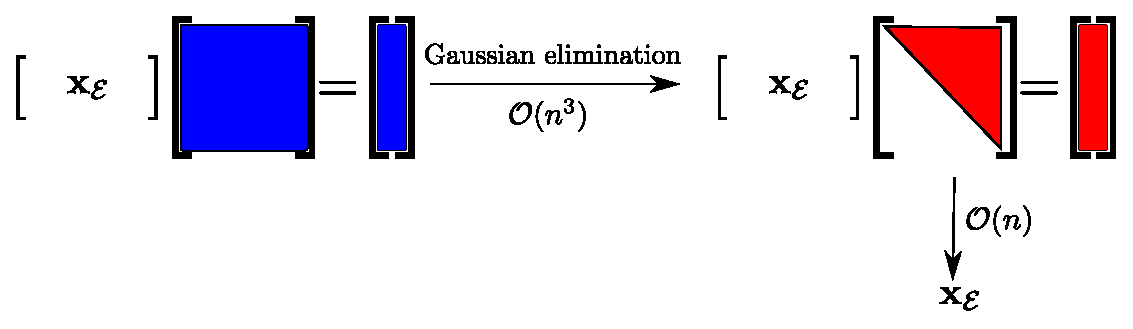
\includegraphics[scale=0.5]{Figuras/Gauss.eps}
\end{center}


}

\frame{
\frametitle{Classic channel coding theory}


\begin{itemize}
\item Decoding via optimal Maximum Likelihood/Maximum a posteriori rules.
\end{itemize}
\begin{itemize}
\item Design the code such that the performance of optimal decoding is as good as possible. 
\end{itemize}
\begin{itemize}
\item Strong algebraic structure so that optimal decoding can be solved more efficiently.
\end{itemize}
\begin{itemize}
\item Small sizes (otherwise decoding complexity becomes prohibitive). 
%We cannot operate very close to capacity at vanishing error probability.
\end{itemize}
\begin{itemize}
\item Linear Block codes (BCH codes, Reed Solomon Codes), Convolutional codes...
\end{itemize}

}

\section{Modern Coding Theory in a nutshell}

\frame{
\frametitle{Modern Coding Theory in a nutshell}

\begin{itemize}
\item Optimal decoding restrains the codes we can use in practice. 
\end{itemize}

\begin{itemize}
\item Our goal is to operate very close to capacity at vanishing error probability.  \textbf{We need to use very long codes!}
\end{itemize}



\begin{block}{Modern capacity-achieving codes}
\begin{itemize}
\item Turbo Codes, LDPC codes, Polar Codes.
\item Approximate decoding. \textbf{Worse than optimal decoding, but much less complex}.
\item Approximate decoding complexity: $\O(n)$.
\item Codes are optimized so that sub-optimal decoding is enhanced!
\end{itemize}
\end{block}

}


\frame{
\frametitle{A suboptimal decoder for linear block codes over the BEC}

\begin{block}{}
Assume the system is already triangularized and reveal as much  information you can.
\end{block}

\begin{itemize}
\item Hamming $(7,4)$ code.
\item $\x=\left[
\begin{array}{ccccccc}
1 & 1 & 1 & 0 & 0 & 0 & 0
\end{array}
\right]$
is sent.
\item $\y=\left[
\begin{array}{ccccccc}
1 & ? & 1 & 0 & ? & ? & 0
\end{array}
\right]$ is received.
\end{itemize}


\begin{columns}
\begin{column}{0.3\textwidth}
\begin{align*}
&x_5=0\\
&x_5\oplus x_6=0\\
&x_2\oplus x_6=1
\end{align*}
\end{column}
\begin{column}{0.7\textwidth}
\begin{center}
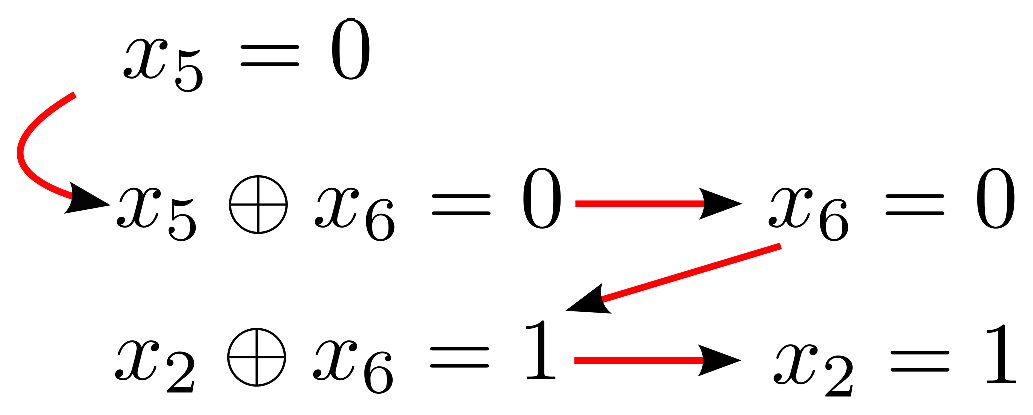
\includegraphics[scale=0.30]{Figuras/approx.eps}
\end{center}
\end{column}
\end{columns}

\begin{exampleblock}{}
The complexity is $\O(n)$!!
\end{exampleblock}


}

\frame{


\begin{itemize}
\item Hamming $(7,4)$ code.
\item $\x=\left[
\begin{array}{ccccccc}
1 & 1 & 1 & 0 & 0 & 0 & 0
\end{array}
\right]$
is sent.
\item $\y=\left[
\begin{array}{ccccccc}
? & 1 & ? & 0 & 0 & ? & ?
\end{array}
\right]$ is received.
\end{itemize}

\begin{align*}
&x_1\oplus x_3\oplus x_7=0\\
&x_3\oplus x_6 \oplus x_7=0\\
&x_6\oplus x_7=0
\end{align*}

\begin{block}{Approximate decoder}
There are no equations with a single variable. No information can be revealed.
\end{block}

\begin{exampleblock}{Optimal decoder}
$x_3$ is revealed ($x_3=0$) by adding the last two equations.
\end{exampleblock}

}

\frame{
\frametitle{A message-passing description}
\begin{align*}
\H=\left[
\begin{array}{ccccccc}
1 & 0 & 1 & 0 & 1 & 0 & 1\\
0 & 1 & 1 & 0 & 0 & 1 & 1 \\
0 & 0 & 0 & 1 & 1 & 1 & 1
\end{array}
\right]
\end{align*}

Tanner graph of the code:

\begin{center}
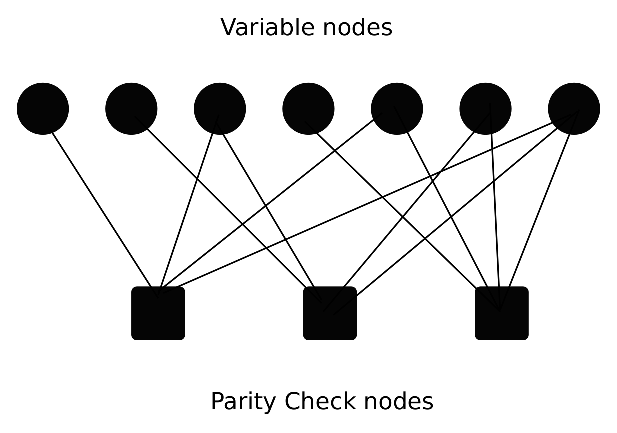
\includegraphics[scale=0.5]{Figuras/tanner47.eps}
\end{center}

}

\frame{
\frametitle{A message-passing description. The BP decoder.}

Initialization: Variable nodes send the channel observation to the parity check nodes they are connected:

\begin{center}
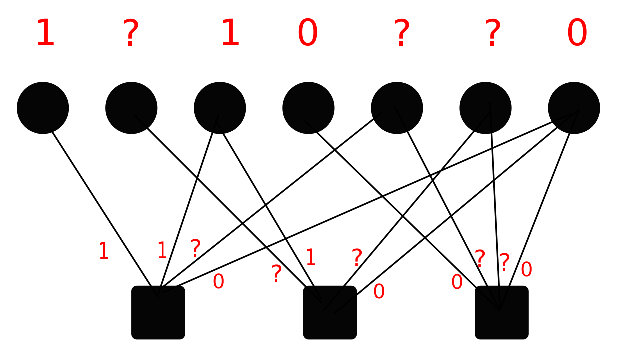
\includegraphics[scale=0.6]{Figuras/tanner47_2.eps}
\end{center}

At each iteration:

\begin{enumerate}
\item Using the received information, each factor tries to resolve the value of the variables that sent a ``?" message. If so, they send the value obtained. Otherwise they send a ``?" message.
\item \textbf{Only factor nodes with a single unknown can resolve a variable!}
\item Variable nodes send their new value or they resend a``?" message.
\end{enumerate}


}

\frame{
\begin{center}
\includegraphics[scale=0.4]{Figuras/1.png}
\end{center}

\begin{center}
\includegraphics[scale=0.23]{Figuras/3.png}
\end{center}

}

\frame{
\begin{center}
\includegraphics[scale=0.16]{Figuras/4.png}
\end{center}

\begin{center}
\includegraphics[scale=0.16]{Figuras/5.png}
\end{center}

}

\frame{
\begin{center}
\includegraphics[scale=0.2]{Figuras/6.png}
\end{center}
%
%\begin{center}
%\includegraphics[scale=0.16]{Figuras/7.png}
%\end{center}

}

\frame{
\frametitle{Sub-optimal decoding for an arbitrary code}
\begin{itemize}
%\item In general, the performance obtained with the suboptimal decoder is quite poor.
\item Given a parity check matrix $\H$ of dimensions $(n-m)\times n$, the number ones per row can be as high as $n$.
\end{itemize}
\begin{itemize}
\item If a row has $\lfloor\alpha n\rfloor$ ones, where $\alpha\in(0,1)$, then the probability that $\lfloor\alpha n\rfloor-1$ of the variables are correctly received and only one is unknown is
\begin{align*}
(\lfloor\alpha n\rfloor)\epsilon(1-\epsilon)^{(\lfloor\alpha n\rfloor-1)}
\end{align*}
which tends to 0 as $\n\rightarrow\infty$.
\end{itemize}
\begin{itemize}
\item \textcolor{darkblue}{Matrix $\H$ has to be carefully designed!}
\end{itemize}



}

\section{Low-density Parity-Check codes}

\frame{
\frametitle{Low-density Parity-Check codes}
LDPC codes: linear block codes defined by \textcolor{darkblue}{sparse parity-check matrices}.
%\begin{align}\nn
%\mathbf{H}_{(\n-m)\times \n},\qquad \mathbf{x}\mathbf{H}^T=\mathbf{0} \;\; \forall  \mathbf{x}\in\mathcal{C}
%\end{align}
%$\n$ is the code length and $\rate=1-\frac{m}{\n}$ is the code rate.


\begin{block}{LDPC (3,6) with $\n=20$}
\begin{figure}
\centering\includegraphics[scale=0.65]{Figuras/H3620.pdf} \hspace{2cm} \centering\includegraphics[scale=0.65]{Figuras/TannerH3620.pdf}
\end{figure}
The density of ones in the matrix $\mathbf{H}$ is $6/\n$ and the rate is $\rate=0.5$.
\end{block}

}

\frame{
\frametitle{Suboptimal decoder using $(3,6)$-LDPC codes. \\ Initialization after BEC transmission}
\begin{itemize}
\item If the number of ones per row is fixed to 6, then the probability that each row in $\mathbf{H}$ has a single unknown is
\begin{align*}
6\epsilon (1-\epsilon)^5
\end{align*}
\textbf{which does not vanish with $\n$!}
\item Let $r_1(0)$ be the fraction of rows in the system of equations with a single unknown. 
\item Note that $r_1(0)\sim \mathcal{B}(6\epsilon (1-\epsilon)^5,(1-\rate)\n)$ and hence
\begin{align*}
\mathbb{E}[r_1(0)]&=\frac{ 6\epsilon (1-\epsilon)^5 (1-\rate)\n}{(1-\rate)\n}=6\epsilon (1-\epsilon)^5 (1-\rate)\n\\
\\
\text{Var}[r_1(0)]&=\frac{ 6\epsilon (1-\epsilon)^5 (1-6\epsilon (1-\epsilon)^5) (1-\rate)\n}{(1-\rate)^2\n^2}=\frac{6\epsilon (1-\epsilon)^5 (1-6\epsilon (1-\epsilon)^5)}{(1-\rate)\n}
\end{align*}
\end{itemize}
}

%\frame{
%\frametitle{Suboptimal decoder using $(3,6)$-LDPC codes. \\ First Iteration}
%\begin{itemize}
%\item $r_1(0)$ variables are revealed because they are connected to parity-check rows with a single unknown.
%\end{itemize}
%\begin{itemize}
%\item As $\n\rightarrow\infty$, it is easy to prove that:
%\begin{enumerate}
%\item Almost all the revealed variables are connected to different parity-check rows.
%\item Consequently, $\mathcal{O}(\n)$ rows with a single unknown will be created. Decoding can proceed!
%\item The whole process can be analytically predicted. This is the key to design capacity-achieving LDPC codes.
%\end{enumerate}
%\end{itemize}
%}



%
%\frame{
%
%\begin{alertblock}{Initialization}
%
%\end{itemize}
%\end{alertblock}
%
%\begin{exampleblock}{During suboptimal decoding}
%\begin{itemize}
%\item Every time a variable is revealed, there is a non-zero probability that a new row with a single unknown is created.
%\item This probability does not depend on $\n$!
%\end{itemize}
%\end{exampleblock}
%
%}
%
%\section{Project 1}
%
%\frame{
%\frametitle{BP vs Optimum ML decoder}
%
%\begin{itemize}
%\item Simulate a BEC channel.
%\item Hamming (7,4) code, encoding the data bits using the generator matrix.
%\item (3,6) LDPC code with $\n=250, 500, 1000$ and $5000$ bits. \textbf{Only $\mathbf{H}$ matrix!}. No encoding, we use the all-zero codeword.
%\item To simulate the optimum ML, use the function {\tt galoislinequations.m}
%\item Obtain plots, interpret results.
%\end{itemize}
%
%
%
%
%}






\frame{
\frametitle{Density evolution for the $(3,6)$ ensemble over the BEC}
\begin{itemize}
\item Assume the code length $\n\rightarrow\infty$.
\item All-zero codeword.
\end{itemize}

\begin{block}{Asymptotic graph}
\begin{itemize}
\item In the limit $\n\rightarrow\infty$, the graph looks like a tree! (the probability of any cycle of finite length in the code tends to zero).
\item Messages received by each node per iteration are independent random variables.
\item We can easily compute the asymptotic evolution of $x^{\ell}$ as the BP iterates.
\end{itemize}                 


\end{block}


}

\frame{
\frametitle{Computation graph for the $(2,4)$ LDPC ensemble}

\begin{itemize}
\item Computation graph: unroll dependencies for a single variable up to a certain level of deepness. 
\end{itemize}
\begin{figure}
\centering\includegraphics[scale=0.5]{Figuras/tree2.png}
\caption{Possible realizations of the depth-1 computation graph for the $(2,4)$ LDPC ensemble, together with their probabilities for a graph generated at random and the probability that the root variable is erased after one iteration of the suboptimal decoder.}
\end{figure}
}





\frame{
\frametitle{Density evolution for the $(3,6)$ ensemble over the BEC}
\begin{itemize}
\item Initialization: variable nodes send an erasure message with probability $\epsilon$. 
\item Let $x^{\ell}$ be the expected probability of an erasure message at iteration $\ell$. Thus, $x^{0}=\pe$.
\item Given $x^{\ell-1}$, using the message-passing update rules for the BEC, we get
\begin{align*}
x^{\ell}=\pe(1-(1-x^{\ell-1})^5)^2
\end{align*}
\end{itemize}

\begin{figure}
\centering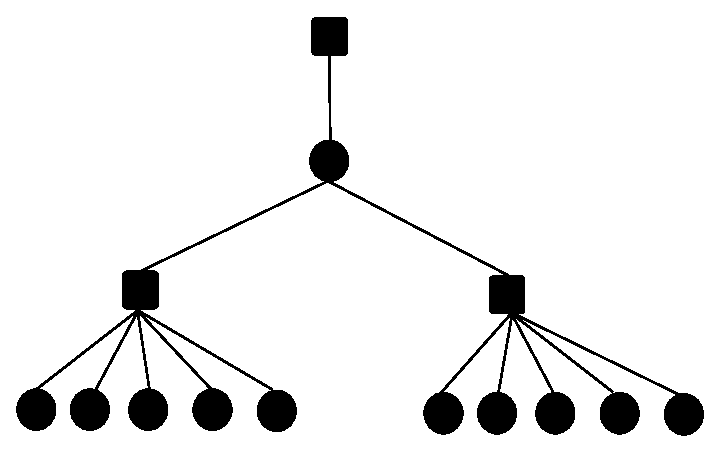
\includegraphics[scale=0.5]{Figuras/tree_36.eps}
\end{figure}


}



\frame{
\frametitle{$(3,6)$ LDPC ensemble's threshold}

\begin{itemize}
\item Using the DE analysis, we can predict if in the asymptotic limit $\n\rightarrow\infty$ the BP is able to successfully decode.
\item Successful decoding: $\lim_{\ell\rightarrow\infty} x^{\ell} =0$.
\end{itemize}

\begin{exampleblock}{}
\begin{align*}
\lim_{\ell\rightarrow\infty} &x^{\ell}\rightarrow0\qquad \pe< 0.4294\\
\lim_{\ell\rightarrow\infty} &x^{\ell}\rightarrow\delta \qquad  \pe\geq0.4294
\end{align*}
where $\delta>0$.
\end{exampleblock}

\begin{block}{}
\textbf{The $(3,6)$ LDPC ensemble cannot operate close to capacity! The threshold is at $0.4294$ while the Shannon limit is at $\epsilon=0.5$.}
\end{block}


}

\frame{
Bit-error rate of the $(3,6)$ ensemble over the BEC $\n=2^{8}$ $(\circ)$, $\n=2^{9}$ $(\square)$ and $\n=2^{11}$ $(\rhd)$.
\begin{figure}
\centering\includegraphics[scale=0.45]{Figuras/errorcurvesv2.pdf}
\end{figure}

\begin{alertblock}{}
The threshold $\pe^*$ can be computed analytically. \textbf{It only depends on the connectivity pattern in the matrix $\mathbf{H}$!}
\end{alertblock}
}


\frame{
\frametitle{What about the error floor?}

\begin{itemize}
\item Error floor is caused by short cycles in the graph. 
\item As an example, let's analyze the error floor caused by codewords of weight $2$ in the (3,6)-LDPC ensemble (generated at random).
\item \textbf{\textcolor{darkblue}{A weight-$2$ codeword exists if the LDPC graph contains the following cycle}}
\end{itemize}

\begin{figure}
\centering\includegraphics[scale=0.3]{Figuras/cycle.png}
\end{figure}

}

\frame{

\begin{itemize}
\item $(3,6)$-LDPC ensemble.
\item Code sample $\mathcal{C}$ is chosen randomly with a uniform probability from the ensemble.
\item Let $N_2$ be the number of codewords with Hamming weight $2$. 
\begin{align*}
N_2\sim \text{Poisson}(\lambda), \qquad \lambda=\frac{375/9}{\n}
\end{align*}
\item The fraction of codes in the ensemble with $N_2=0$ is $\exp^{-\lambda}$.
\item The average bit error rate caused by codewords with Hamming weight $2$ is
\begin{align*}
P_b \approx 2 \epsilon^2 \frac{375/9}{\n}
\end{align*}
\end{itemize}



\textbf{Proof:}
For a given pair of variables, the probability that they are connected to the same 3 parity check nodes is 
\begin{align*}
p_2=3\frac{5}{3n-3}\frac{5}{3\n-4}\frac{5}{3\n-5}\approx \frac{375/9}{\n^3}
\end{align*} 
Since there are $\n^2$ pairs of variables, then $\mathbb{E}[N_2]=\frac{375/9}{\n}$. Then, $N_2\sim \mathcal{B}(p_2,\n^2)$, which tends with $\n$ to $N_2\sim \text{Poisson}(\frac{375/9}{\n})$. Therefore, $P(N_2==0)=\exp(-\lambda)$.

}

\section{Irregular LDPC codes}

\frame{
\frametitle{Regular LDPC codes of rate $1/2$}

\begin{center}
\begin{tabular}{|cccc|}
\hline
$l$ & $r$ & $\rate$ & $\pe^*$ \\
\hline
3 & 6 & 1/2 & 0.43 \\
4 & 8 & 1/2 & 0.38 \\
5 & 10 & 1/2 &  0.34\\
\hline
\end{tabular}
\end{center}

Increasing the density does not help...
}


\frame{
\frametitle{Irregular LDPC codes}

\begin{itemize}
\item Improving the  solution in the asymptotic  limit $\n\rightarrow\infty$ by \textbf{optimizing the LDPC graph degree distribution (DD).}
\item LDPC ensemble: set of codes of length $\n$ that exhibit the same DD in the Tanner graph.
\end{itemize}
\begin{itemize}
\item \textbf{Variable perspective DD:}
\begin{itemize}
	\item $L_i$ Fraction of variables with  degree $i$.
	\item $R_j$ Fraction of check nodes with degree $j$.
\end{itemize}
\end{itemize}
\begin{itemize}
\item \textbf{Edge perspective DD:}
\begin{itemize}
	\item $\lambi{i}$ Fraction of edges with left degree $i$.
	\item $\rhi{j}$ Fraction of edges with right degree $j$.
\end{itemize}
\end{itemize}
}

\frame{

\begin{itemize}
\item DD is typically given in polynomial form
\begin{align*}
\lambfull, \;\; \rhofull. 
\end{align*}
\end{itemize}
\begin{itemize}
\item The \emph{design rate} of the code is 
\begin{align*}
\rate=1-\frac{\int_{0}^{1}\rho(x)dx}{\int_{0}^{1}\lambda(x)dx} 
\end{align*}
\item The density of the matrix
\begin{align*}
\Delta=\frac{1}{\int\lambda(x)}\frac{1}{\rate}
\end{align*}
measures the complexity of the ensemble (edges per information bit).
\end{itemize}
}

\frame{
\frametitle{An example}

Consider the DD:
\begin{align*}
\lambda(x)=x,  ~~~~~~~~~~~ \rho(x)=\frac{x^3}{3}+\frac{2~x^4}{3}
\end{align*}

\begin{itemize}
\item All edges have degree $2 \Rightarrow$ all variable nodes (n) have degree 2.
\item The graph contains $\frac{1}{3}\frac{2n}{4}=\frac{n}{6}$ check nodes of degree 4 and $\frac{2}{3}\frac{2n}{5}=\frac{4n}{15}$ check nodes of degree 5. 
\item The average check node degree is
\begin{align*}
R_{\text{avg}}&=4\frac{n/6}{n/6+4n/15}+5 \frac{4n/15}{n/6+4n/15}\approx 4.6153
\end{align*} 
and can be computed as $\left(\int_0^1 \rho(x) dx\right)^{-1}$.
\item The rate of the code is
\begin{align*}
\rate=1-\frac{\text{\# rows in $\H$}}{\text{\# columns in $\H$}}=1-\frac{\frac{2n}{R_{\text{avg}}}}{n}\approx 0.5667
\end{align*}
\end{itemize}

}



\frame{
\frametitle{Density evolution over the BEC}

\begin{itemize}
\item For any given ensemble DD defined by its degree distribution pair $\lambda(x)$ and $\rho(x)$, we can easily generalized the DE recursion.
\end{itemize}

\begin{align*}
\text{\textbf{Density Evolution (DE):}     }x_{\ell}=\epsilon\lambda(1-\rho(1-x_{\ell-1}))   , 
\end{align*}

\begin{block}{Degree distribution LDPC optimization}
For a fixed rate $\rate$, optimize the coefficients of $(\lambda(x),\rho(x))$ to obtain a threshold close to channel capacity.
\end{block}

}



\frame{



If we fix the maximum left degree to $l_{max}=100$, the rate $\rate=1/2$ and we set a constant check node degree $\rho(x)=x^{10}$. 
\begin{block}{}
\begin{align*}
\lambda(x)&=0.169010x+0.162144x^{2}+0.005938x^{4}+0.016799x^{5}+0.186455x^{6}\nonumber\\&+0.006864x^{13}+0.025890x^{16}+0.096393x^{18}+0.010531x^{26}\nonumber\\&+0.004678x^{27}+0.079616x^{28}+0.011885x^{38}+0.224691x^{99}.
\end{align*}
\end{block}
\begin{itemize}
\item For the BEC,  the BP threshold is $\pe^*\approx0.485$.
\item In the AWGN channel, the gap to capacity is only $0.02370$ dB.
%\item \textbf{Is this the end of coding theory? Are irregular LDPC codes the final solution?}  
\end{itemize}
}

\begin{frame}{Irregular LDPC codes in practice. Drawbacks.}
\small{
\begin{itemize}
\item Gap to capacity only vanishes in the limit $l_{max}\rightarrow\infty$.
\item Irreducible error floor (even for the optimal decoder). Stopping sets!
\item \color{red}{\textbf{Strong trade-off between performance in the waterfall region and error floor.}}
\end{itemize}
}
\begin{columns}[T]
\begin{column}{0.5\textwidth}
\begin{figure}[htbp]
\includegraphics[scale=0.3]{Figuras/Olmos_CL2010-2015_fig4.pdf} 
\end{figure}
\small{\color{red}{\textbf{The $(3,6)$ regular code has $\pe^*=0.4294$ but no error floor...}}.} 
\end{column}
\begin{column}{0.5\textwidth}
\small{
\begin{align}
\rho(x)&=x^{5}\nonumber\\
\lambda(x)&=0.416x+0.166x^{2}+0.1x^{3}+0.07x^{4}+0.053x^5\nonumber\\&+0.042x^{6}+0.035x^{7}+0.03x^{8}+0.026x^{9}\nonumber\\&+0.023x^{10}+0.02x^{11}+0.0183x^{12},\nonumber\\
\pe^*&=0.4808, \quad\quad  \rate=1/2 \nonumber 
\end{align}}
\begin{figure}[htbp]
\includegraphics[scale=0.4]{Figuras/SS.pdf} 
\caption{SS of weight two}.
\end{figure}
\end{column}
\end{columns}
\end{frame}


\section{Convolutional LDPC codes}


\frame{
\frametitle{Capacity-achieving codes}

\begin{itemize}
\item Polar Codes.
\item LDPC Convolutional codes (spatially-coupled LDPC codes).
\end{itemize}


\begin{block}{}
Irregular LDPC codes theoretically achieve channel capacity but they are very hard to implement in VLSI circuits.
\end{block}

\begin{block}{}
\begin{itemize}
\item Most of actual and next generation communication standards only consider quasi-regular LDPC codes.
\item Regular LDPC codes can be efficiently implemented (area, energy, throughput,...).
\end{itemize}
\end{block}

}

\frame{
\frametitle{LDPCC  based on the $(3,6)$-regular LDPC codes}

\begin{itemize}
\item $L$ independent $(3,6)$-regular LDPC codes  of length $M$ bits are linked in a deterministic way. \end{itemize}


\begin{figure}[!ht]
\centering
\includegraphics[scale=0.4]{Figuras/uncchain36}
\end{figure}
We connect each variable node to a random check node of the code in the left and the code in the right
\begin{columns}[T]
\begin{column}{0.5\textwidth}
\begin{figure}[!ht]
\centering
\includegraphics[scale=0.5]{Figuras/cchain36}
\end{figure}
\end{column}
\begin{column}{0.5\textwidth}
\begin{itemize}
\item $L$ is the chain length. $ML$ is the total codelength.
\item For $L\rightarrow\infty$ the code looks like a $(3,6)$ ensemble....
\item Low-degree check nodes in the boundaries, higher protection!
\end{itemize}
\end{column}
\end{columns}


}




\frame{

\begin{columns}[T]
\begin{column}{0.5\textwidth}
\begin{center} $\mathbf{H}$ matrix for $L=20$ and $M=1024$\end{center}
\begin{figure}[!ht]
\centering
\includegraphics[scale=0.3]{Figuras/Hcoupled}
\end{figure}

\end{column}
\begin{column}{0.5\textwidth}
\vspace{0.5cm}

\begin{itemize}
\item[] The rate of the code is 
\end{itemize}
\begin{equation}
\rate(3,6,L)=\frac{1}{2}-\underbrace{\frac{1}{L}}_{\text{rate loss!!}} \nonumber
\end{equation}
\textbf{\textcolor{red}{We need $L$ to be very large!}}
\end{column}
\end{columns}

%\begin{itemize}
%\item The BP threshold of the uncoupled $(3,6)$-LDPC ensemble is $0.4294$.
%\item For $L\rightarrow \infty$, the LPDCC code has rate $\rate(3,6,L)\approx 1/2$.
%\item It's BP threshold rises up to $0.48815\approx \pe_{MAP}(3,6)$ (capacity is achieved at 0.5!).
%\end{itemize}


}

\frame{
\beamertemplatetransparentcoveredhigh
\frametitle{Density Evolution}
\begin{itemize}
\item DE recursion can be generalized to the convolutional ensemble .
\item Surprisingly, the BP threshold $\pe^*(3,6,L)$ outperforms the BP limit for the $(3,6)$ code and tends to the optimal threshold $\pe^{opt}(3,6)\approx0.4881$.
\item Much closer to capacity!
\item \color{red}{\textbf{ $\pe^*(5,10,L=50)=0.499486$!}}
\end{itemize}

\begin{center}
\begin{tabular}{|ccccc|}
\hline
$l$ & $r$ & $\rate$ & $\pe^*$ & $\pe^*(l,r,L)$ \\
\hline
3 & 6 & 1/2 & 0.43 & 0.48815 \\
4 & 8 & 1/2 & 0.38 & 0.4947 \\
5 & 10 & 1/2 &  0.34 & 0.4994\\
\hline
\end{tabular}
\end{center}
}




\frame{
\frametitle{Decoding the $(3,6)$ convolutional ensemble}

Above the uncoupled $(3,6)$ code threshold, $\pe\geq 0.4294$, the code is peeled off from the boundaries towards the center of the code

\begin{figure}[h]
\centering
\begin{tabular}{cc}
\includegraphics[width=3cm]{Figuras/L_20_M_512_Iter_5} & \includegraphics[width=3cm]{Figuras/L_20_M_512_Iter_30} \\  \includegraphics[width=3cm]{Figuras/L_20_M_512_Iter_70} & \includegraphics[width=3cm]{Figuras/L_20_M_512_Iter_110} 
\end{tabular}
\end{figure}

}

\frame{
\frametitle{Windowed decoding}
\small{
\begin{itemize}
\item LDPCC codes are in general quite large because both $M$ and $L$ are as big as possible.
\item One solution to reduce complexity further is to use a fixed sized window (of small size compared to $L$) to perform decoding.
\item This also results in a reduced decoding latency and could be used in latency constrained applications.
\item Moreover, spatially coupled codes with $L = \infty$ (convolutional-like codes) can only be decoded through such a windowed decoder.
\end{itemize}
}
\begin{figure}[!ht]
\centering
\includegraphics[scale=0.5]{Figuras/wd}
\caption{To decode variables in the first section, we use a subgraph involving sections $1,\ldots,W$}. 
\end{figure}
}


\end{document}

